\section{MiCS Internal Workflow} % (fold)
\label{sec:workflow_overview}

This section provides a brief overview of how MiCS works. Figure \ref{fig:mics_internal_workflow} shows the stages that MiCS goes through when converting C\# to JavaScript.

\begin{figure}[H]
	\begin{center}
		\centerline{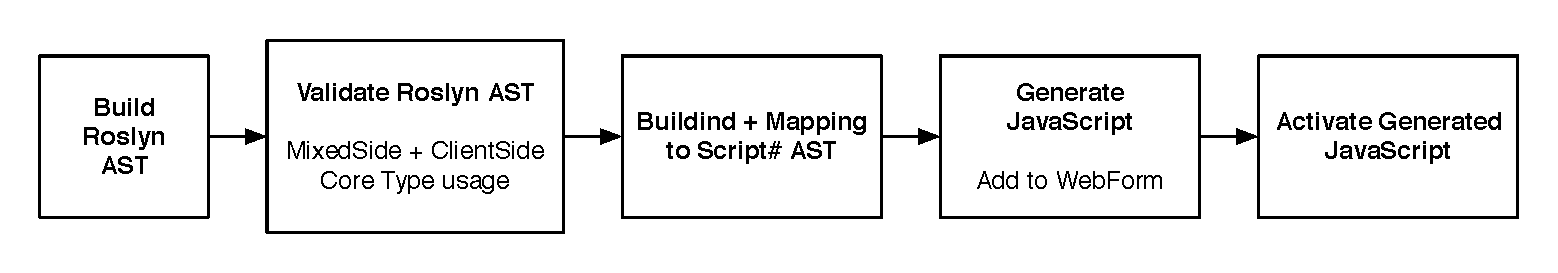
\includegraphics[width=18cm]{resources/images/internalworkflow.eps}}
	\end{center}
	\caption{MiCS Internal Workflow}
	\label{fig:mics_internal_workflow}
\end{figure}

TODO: Update figure

MiCS uses Roslyn to generate a C\# AST representing the developer's  C\# code. 

When the Roslyn AST has been obtained it needs to be validated to ensure that the written code complies with the Mixed Side Principle and that core types are only used in a supported manner. Without validation, it would be possible for the user to generate incorrect JavaScript.

Once the AST has been validated, it is ready to be mapped to the Script\# AST. This is the core functionality of MiCS - transforming a Roslyn AST to a Script\# AST. During the mapping process it is checked that the user does not utilize any C\# constructs that is not support by MiCS. 

When the Roslyn AST has successfully been mapped to a Script\# AST, MiCS utilizes Script\#’s built-in \texttt{ScriptGenerator} to generate the JavaScript corresponding to the developers’s original C\# code. 

When JavaScript has been generated, it needs to be embedded into the developer’s web page. Code that calls client side event handlers also needs to be generated so that the JavaScript will be executed.


% section workflow_overview (end)